
%remark 

\begin{theorem}[Tunnel Troll Theorem]
Let $\Xi$ be a deterministic unary oritatami system of delay $\delta = 1$. The following statements hold.
\begin{enumerate}
\item At arity $\alpha \geq 3$, if $S[i] = t$ (i.e. the tunnel that stabilizes $w[i]$ is not singular) and $S[i+1] \neq \blacksquare$, then $\#bc(C_{i-1}) > \#bc(C_i)$.
\item At arity $\alpha = 2$, if $n$ is the number of $bt$ in $S[i..j]$ for some $i,j$ such that $S[i] = b$ and $i < j$, then $\#bc(C_{i-2}) - \#bc(C_{j}) \geq n$.
\end{enumerate}
\end{theorem}

%%%%%%%%%%%%%%%%%%%%%%%%%%%%%%%%%%%%%%%%%%%%%%%%%%%%

\begin{figure}[tb]
  \begin{center}
    \begin{tabular}{ccc}
    
    
      \begin{minipage}{0.3\hsize}
      \centering
        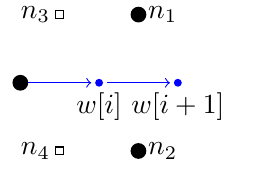
\begin{tikzpicture}
        \draw[->, white] (0:0)--(-120:1);
	 \draw[->,white] (120:0.8)--(120:0.1);%for adjustment
          
            \fill[blue] (0,0) circle [radius=0.05];
            \node[below] at (0,0) {$w[i]$};
            \node[below] at (0:1) {$w[i+1]$};

            \foreach \theta in {0}{
              \fill[transform canvas={shift=(\theta:1)},blue](0,0) circle [radius=0.05];
            }
            
            \foreach \theta in {60,-60,180}{
              \fill[transform canvas={shift=(\theta:1)}](0,0) circle [radius=0.1];
            }

            \foreach \theta in {120,-120}{
              \draw[transform canvas={shift=(\theta:1)}](-0.05,-0.05) rectangle (0.05,0.05);
            }
            
            \draw[->, blue] (180:0.9)--(180:0.1);
            \draw[->, blue] (0:0.1)--(0:0.9);

            \node[transform canvas={shift=(60:1)},right] {$n_1$};
            \node[transform canvas={shift=(-60:1)},right] {$n_2$};
            \node[transform canvas={shift=(120:1)},left] {$n_3$};
            \node[transform canvas={shift=(-120:1)},left] {$n_4$};


         % \node at (0,-2) {$t_{0}$};
        \end{tikzpicture}
      \end{minipage}

      

      \begin{minipage}{0.3\hsize}
      \centering
        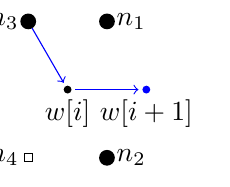
\begin{tikzpicture}
	\draw[->, white] (0:0)--(-120:1);
            \fill(0,0) circle [radius=0.05];
            \node[below] at (0,0) {$w[i]$};
            \node[below] at (0:1) {$w[i+1]$};

            \foreach \theta in {0}{
              \fill[transform canvas={shift=(\theta:1)},blue](0,0) circle [radius=0.05];
            }
            
            \foreach \theta in {60,-60,120}{
              \fill[transform canvas={shift=(\theta:1)}](0,0) circle [radius=0.1];
            }

            \foreach \theta in {180,-120}{
              \draw[transform canvas={shift=(\theta:1)}](-0.05,-0.05) rectangle (0.05,0.05);
            }
            
            \draw[->, blue] (120:0.9)--(120:0.1);
            \draw[->, blue] (0:0.1)--(0:0.9);

            \node[transform canvas={shift=(60:1)},right] {$n_1$};
            \node[transform canvas={shift=(-60:1)},right] {$n_2$};
            \node[transform canvas={shift=(120:1)},left] {$n_3$};
            \node[transform canvas={shift=(-120:1)},left] {$n_4$};
            \node[transform canvas={shift=(180:1)},left] {$n_5$};

          %\node at (0,-2) {$t_{\pm 60}$};
        \end{tikzpicture}
      \end{minipage}

      \begin{minipage}{0.3\hsize}
      \centering
        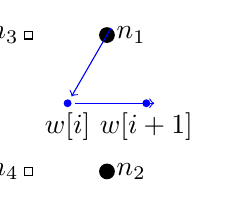
\begin{tikzpicture}
        \draw[->, white] (0:0)--(-120:1);
            \fill[blue](0,0) circle [radius=0.05];
            \node[below] at (0,0) {$w[i]$};
            \node[below] at (0:1) {$w[i+1]$};

            \foreach \theta in {0}{
              \fill[transform canvas={shift=(\theta:1)}, blue](0,0) circle [radius=0.05];
            }
            
            \foreach \theta in {60,-60}{
              \fill[transform canvas={shift=(\theta:1)}](0,0) circle [radius=0.1];
            }

            \foreach \theta in {180,-120,120}{
              \draw[transform canvas={shift=(\theta:1)}](-0.05,-0.05) rectangle (0.05,0.05);
            }
            
            \draw[->, blue] (60:1.1)--(60:0.1);
            \draw[->, blue] (0:0.1)--(0:1.1);

            %\node[transform canvas={shift=(0:1)},below] {$n_0$};
            \node[transform canvas={shift=(60:1)},right] {$n_1$};
            \node[transform canvas={shift=(-60:1)},right] {$n_2$};
            \node[transform canvas={shift=(120:1)},left] {$n_3$};
            \node[transform canvas={shift=(-120:1)},left] {$n_4$};
            \node[transform canvas={shift=(180:1)},left] {$n_5$};

         % \node at (0,-2) {$t_{\pm 120}$};
        \end{tikzpicture}
      \end{minipage}
      
    \end{tabular}
    \caption{Direction into a entrance}
    \label{TTT_tunnel_direction}
  \end{center}
\end{figure}

\begin{lemma}
\label{TTT_entrance_Tab}
Let $\Xi$ be a deterministic unary oritatami system at delay $\delta = 1$, arity $\alpha =2$. 
Assume $\Xi$ stabilizes the transcript until $w[i-1]$. If $S[i+1] = b$ and $S[i+2] \in \{ t_s, t_o \} $, then $\#bc(C_{i-1}) > \#bc(C_{i})$.
\end{lemma}

\begin{proof}%[lemma \ref{TTT_entrance_Tab}]
See Fig.\ref{TTT_tunnel_direction}.
$S[i+2] \in \{ t_s, t_o \} $ means that $w[i+2]$ is stabilized by a tunnel section of type $S$ or $O$.
Thus,  its predecessor $w[i+1]$ must be inside the tunnel section, that is, $n_1$ and $n_2$ must be occupied.
Free bonds of $w[i]$, if any, cannot be used in future by another bead $w[j]$ because otherwise the part of transcript $w[i..j]$ and the bond between $w[i]$ and $w[j]$ would form a closed curve and the curve would cross the path of $C_{i-1}$ between $n_1$ and $n_2$, contradiction.
%Binding capabilities that $w[i]$ supplies are inactive according to Jordan curve theorem on $n_1$, $n_2$, and $w[i]$.
Therefore, if $w[i]$ forms a bond at its stabilization $\#bc(C_{i-1}) > \#bc(C_{i})$ holds.
We now prove that $w[i]$ must form a bond.


Suppose $w[i]$ were stabilized without any bond, that is, by a tunnel.
For that the two points that are a neighbor of both $w[i-1]$ and $w[i]$ must be occupied already.
In addition, at least one of the neighbors of $w[i]$ must be free because $S[i+1] = b$.
Thus, only the case to be considered is Fig.~\ref{TTT_tunnel_direction} (middle) with $n_5$ being occupied (that is, $n_4$ is free).
In this case, before $w[i]$ is stabilized, at lest three neighbors of $n_2$ were free and hence, a bead at $n_2$ was provided with one free bond and could form a bond with $w[i]$. \qed




\end{proof}


%%%%%%%%%%%%%%%%%%%%%%%%%%%%%%%%%%%%%%%%%%%%%%%%%%%%
\begin{figure}[tb]
  \centering
    \begin{tabular}{cc}
    \centering
      \begin{minipage}{0.45\linewidth}
      \centering
        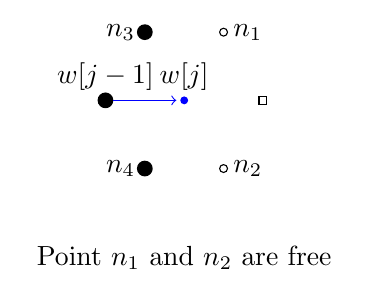
\begin{tikzpicture}
	\draw[white] (0:0) -- (120:1);
	\draw[white] (0:0) -- (-60:1);
	\draw[white] (0:0) -- (0:1);

            \fill[blue](0,0) circle [radius=0.05];
            \node[above] at (0,0) {$w[j]$};

            
            \foreach \theta in {120,-120,180}{
              \fill[transform canvas={shift=(\theta:1)}](0,0) circle [radius=0.1];
            }

            \foreach \theta in {0}{
              \draw[transform canvas={shift=(\theta:1)}](-0.05,-0.05) rectangle (0.05,0.05);
            }
            \draw (-60:1) circle [radius=0.05];
            \draw (60:1) circle [radius=0.05];

            \draw[->, blue] (180:0.9)--(180:0.1);



            \node[transform canvas={shift=(60:1)},right] {$n_1$};
            \node[transform canvas={shift=(-60:1)},right] {$n_2$};
            \node[transform canvas={shift=(120:1)},left] {$n_3$};
            \node[transform canvas={shift=(-120:1)},left] {$n_4$};
            \node[transform canvas={shift=(180:1)},above] {$w[j-1]$};

          \node at (0,-2) {Point $n_1$ and $n_2$ are free};
        \end{tikzpicture}
      \end{minipage}

      \begin{minipage}{0.45\linewidth}
      \centering
        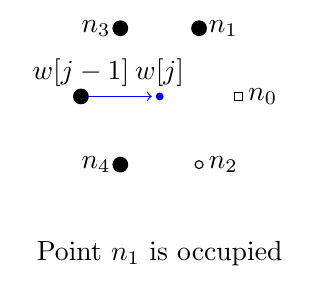
\begin{tikzpicture}
	\draw[white] (0:0) -- (0:1);
	\draw[white] (0:0) -- (120:1);
	\draw[white] (0:0) -- (-90:2);

            \fill[blue](0,0) circle [radius=0.05];
            \node[above] at (0,0) {$w[j]$};
            
            \foreach \theta in {120,-120,180,60}{
              \fill[transform canvas={shift=(\theta:1)}](0,0) circle [radius=0.1];
            }

            \foreach \theta in {0}{
              \draw[transform canvas={shift=(\theta:1)}](-0.05,-0.05) rectangle (0.05,0.05);
            }
            \draw (-60:1) circle [radius=0.05];

            \draw[->, blue] (180:0.9)--(180:0.1);

            \node[transform canvas={shift=(0:1)},right] {$n_0$};
            \node[transform canvas={shift=(60:1)},right] {$n_1$};
            \node[transform canvas={shift=(-60:1)},right] {$n_2$};
            \node[transform canvas={shift=(120:1)},left] {$n_3$};
            \node[transform canvas={shift=(-120:1)},left] {$n_4$};
            \node[transform canvas={shift=(180:1)},above] {$w[j-1]$};


          
          \node at (0,-2) {Point $n_1$ is occupied};
        \end{tikzpicture}
      \end{minipage}
    \end{tabular}
    \caption{Exit of Tunnel}
    \label{TTT_tunnel_exit}
\end{figure}


\begin{lemma}
\label{TTT_exit}
Let $\Xi$ be a deterministic unary oritatami system of delay $\delta = 1$ and arity $\alpha =2$.
%Let $w[i]$ be a bead which is stabilized at the exit of a tunnel.
If $S[i+1..j+1] = bt^{(j-i-1)}b$ for some $i,j$ with $i \leq j-2$ and $S[j] \in \{ t_s, t_o\}$, then $\#bc(C_{j-2}) \geq \#bc(C_j)$, and hence, $\#bc(C_{i}) \geq \#bc(C_j)$.
If $i \leq j-3$, then the second inequality is strengthened as $\#bc(C_{i}) > \#bc(C_{j})$.
%if we assume $\#bc(C_{i-2}) - \#bc(C_{i-1}) = a$, then $\#bc(C_{i}) - \#bc(C_{i-1}) \leq a$.
\end{lemma}

\begin{proof}%[Lemma~ \ref{TTT_exit}]
Since the binding capability never increases inside a tunnel, we just need to consider the exit of a tunnel.
See Fig.\ref{TTT_tunnel_exit}. 
At least one of points $n_1$ or $n_2$ must be free because otherwise $w[j]$ would be inside of a tunnel, that is, $S[j+1]$ would not be $b$.

%If $i - h > 1$ and $j$ is such that $h \leq j<i$, then $\#bc(C_{j-1}) \geq \#bc(C_{j})$ because all neighbors of $w[j]$ are occupied by beads forming the tunnel so that any $w[i+1..]$ cannot reach neighbors of $w[j]$. 
%Thus, inside this tunnel, binding capabilities never increased.


Let $m$ be the number of bonds $w[j-1]$ forms, that is, $\#bc(C_{j-2}) - \#bc(C_{j-1}) = m$.
We claim $\#bc(C_{j}) - \#bc(C_{j-1}) \leq m$.
Indeed, if both $n_1$ and $n_2$ are free (see Fig.~\ref{TTT_tunnel_exit}), the predecessor $w[j-1]$ must be bound to both beads at $n_3$ and at $n_4$ because both of them still have a free hand.
Hence, $m \geq 2$.
Since $\#bc(C_{j}) - \#bc(C_{j-1})$ is less than the arity, this difference is at most $m$.

If $n_1$ is occupied, then $n_2$ is free.
The predecessor $w[j-1]$ must be bound $n_4$.
Hence,  $m \geq 1$.
The bead $w[j]$ can increase the binding capability at most by 1 because one of its free neighbors would, $n_0$ or $n_2$, is to be occupied by the successor $w[j+1]$.
Therefore, $\#bc(C_{j}) - \#bc(C_{j-1}) \leq m$.
  


Thus,$\#bc(C_{j-2}) \geq \#bc(C_j)$ , and hence, $\#bc(C_{i}) \geq \#bc(C_j)$.
If $i \leq j-3$, then the second inequality is strengthened as $\#bc(C_{i}) > \#bc(C_{j})$ because $S[i+1] = b$, that is, $\#bc(C_{i}) > \#bc(C_{i+1})$ and $\#bc(C_{i+1}) \geq \#bc(C_j)$. \qed


\end{proof}

%%%%%%%%%%%%%%%%%%%%%%%%%%%%%%%%%%%%%%%%%%%%%%%%%%%%


\begin{lemma}
\label{TTT_tunnelC_lemma}
Let $\Xi$ be a deterministic unary oritatami system of delay $\delta = 1$, arity $\alpha = 2$.
If $S[i+2] = t_a$, the following statements hold.
\begin{enumerate}
\item If $S[i] = b$, $\#bc(C_{i-1}) > \#bc(C_{i+2})$.
\item If $S[i] \in \{t_s, t_o \}$, $\#bc(C_{i-2}) > \#bc(C_{i+2})$.
\item If $S[i] = t_a$, $\#bc(C_{i-3}) - 2 \geq \#bc(C_{i+2})$.
\end{enumerate}
%If there are indices $i,j$ such that $S[i..j+1]$ is either $bbt^{(j-i-1)}b$ and $S[i+2] = t_a$ or $bt^\ell bt^{j-i-1-\ell}b$ for some $\ell$ and $S[i+l+2] = t_a$, then $\#bc(C_{i-1}) > \#bc(C_j)$.
\end{lemma}


%\begin{lemma}
%\label{TTT_tunnelC_lemma}
%Let $\Xi$ be a deterministic unary oritatami system of delay $\delta = 1$, arity $\alpha = 2$. We assume $S[h..i+1] = bt^{(i-h)}b \quad (1<h<i)$. If at least one of $w[h+1..i]$ is stabilized by tunnel $C$, then $\#bc(C_{h-3}) > \#bc(C_{h+1})$ and $\#bc(C_{h-3}) > \#bc(C_i)$.
%\end{lemma}


%\begin{proof}[Lemma~ \ref{TTT_tunnelC_lemma}]
%Let $\Xi$ be a unary oritatami system at $\delta = 1, \alpha = 2$.
%Assume $S[h..i+1] = bt^{i-h}b (h<i)$. If at least one of $w[h+1..i]$ are stabilized by tunnel $C$, then only $w[h+1]$ can use tunnel $C$ because if $w[g]$ which is one of $w[h+2..i]$, with $h+2 \leq g \leq i$ is stabilized by tunnel $C$, $C_g$ is a terminal.
%
%
%Let us consider stabilization $S[h-1..h+1] = tbt$ or $S[h-1..h+1] = bbt$ as follows. In result, $\#bc(C_{h-3}) > \#bc(C_{h+1})$. In addition according to Lemma~\ref{TTT_exit} $\#bc(C_{h+1}) \geq \#bc(C_{i})$. Thus, $\#bc(C_{h-3}) > \#bc(C_{h+1})$ and $\#bc(C_{h-3}) > \#bc(C_{i})$.
%\\
%
%\subsubsection{Case of $S[h-1..h+1] = bbt$}
%See Fig.~\ref{TTT_tunnelC_enter_usingBond}.
%If $w[h-1]$ forms one bond, then it leaves one free bond, but it is consumed by $w[h+1]$.
%In addition, $w[h]$ has to bound.
%Thus, in this cases, binding capability decreases by 1.
%If $w[h-1]$ forms two bonds, then it does not leave any bond.
%In addition, $w[h]$ has to be bound.
%Thus, in this case, even if $w[h+1]$ supplies two free bonds, binding capability decreases by 1.


\begin{figure}
  \begin{center}
        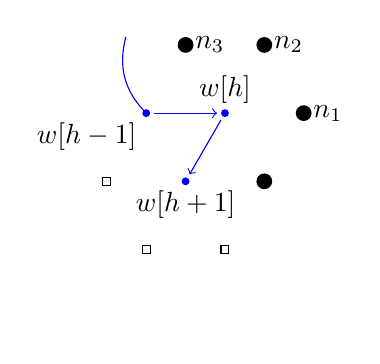
\begin{tikzpicture}
        \draw[->,white] (-70:0.1) -- (-70:3);
          \foreach \theta in {60,-60,120,0}{
            \fill[transform canvas={shift=(\theta:1)}](0,0) circle [radius=0.1];
          }

          \fill[blue](180:1) circle [radius=0.05];
          \fill[blue](0:0) circle [radius=0.05];

          \draw[transform canvas={shift=(180:1)}, blue] (105:1) edge[bend right] (105:0);
          \draw[->, blue] (180:0.9) -- (180:0.1);
          \draw[->, blue] (-120:0.1) -- (-120:0.9);

          \node[below left] at (180:1) {$w[h-1]$};
          \node[above] at (0:0) {$w[h]$};
          \node[below] at (-120:1) {$w[h+1]$};

          \node[right] at (120:1) {$n_3$};
          \node[right] at (60:1) {$n_2$};
          \node[right] at (0:1) {$n_1$};

          \begin{scope}[shift=(-120:1)]
            \fill[blue](0,0) circle [radius=0.05];
            \foreach \theta in {-120,-60,180}{
              \draw[transform canvas={shift=(\theta:1)}](-0.05,-0.05) rectangle (0.05,0.05);
            }
            
          \end{scope}
        \end{tikzpicture}
    \caption{Case of $S[h-1..h+1] = bbt$}
    \label{TTT_tunnelC_enter_usingBond}
  \end{center}
\end{figure}

%\subsubsection{Case of $S[h-1..h+1] = tbt_a$}
%Fig.\ref{TTT_tunnelC_enter_usingTunnel} exhibits all the two kinds of stabilization depending on structures of tunnel C.
%
%%\item{Left of Fig.\ref{TTT_tunnelC_enter_usingTunnel}}\\
%  In this figure, Bead $n_4$ has at least one binding so that $w[h-1]$ has to bound $n_4$. Moreover, $w[h]$ has to bind to one of $n_1, n_2, n_3$ in order to stabilize deterministically. On the other hand, $w[h+1]$ can supply two bindings but has only two free neighbors. One of them is occupied by a successor. Therefore $w[h+1]$ can only bind one of $n_5, n_6$, that is, $w[h+1]$ supplies at most one binding. Thus, this case $\#bc(C_{h-1}) > \#bc(C_{h+1})$.
%
%  These cases are divided on number of capabilities that $w[h-1]$ consumes.
%  \begin{itemize}
%  \item[-]{$w[h-1]$ does not consume any bindings}\\
%  According to Lemma~\ref{TTT_exit}, $\#bc(C_{h-3}) \geq \#bc(C_{h-1})$ because of $S[h-1] = t$.
%    $w[h]$ has to bound one of $n_1, n_2, n_3$ in order to stabilize deterministically so that  $\#bc(C_{h-1}) > \#bc(C_{h})$.
%    $w[h+1]$ has to be bound to $w[h-1]$ because $w[h-1]$ has bindings, that is, $w[h+1]$ consumes at least one hand and supplies at most one hand so that $\#bc(C_{h}) \geq \#bc(C_{h+1})$. Thus, in this cases $\#bc(C_{h-3}) > \#bc(C_{h+1})$.
%%     This time, let us consider either $n_4$ is occupied or not. If $n_4$ is occupied, then $w[h-1]$ has no active bindings that is this situation consumes some binding capabilities. If $n_4$ is free and $w[h+2]$ is stabilized in $n_4$, then $w[h-1]$ has to bind $w[h+2]$. Therefore, In this case, stabilization of $w[h-1..h+2]$ consumes some bindings. If $n_4$ is free and $w[h+2]$ is stabilized except $n_4$, then this oritatami system has to use two binding capabilities in order to bind $w[h+2]$. Therefore, in this case consumes some bindings. Thus in this cases $\#bc(C_{h-1}) > \#bc(C_{h+2})$.
%
%  \item[-]{$w[h-1]$ consumes one binding}\\
%    In this case, $w_{h}$ has to be bound one of $n_1, n_2, n_3$. In addition, $w[h-1]$ and $w[h+1]$ are not supply any bindings. Thus, in this cases consume some binding capabilities.
%  \item[-]{$w[h-1]$ consumes two bindings}\\
%    In this case, $w[h-1]$ already consumes two binding. $w[h]$ has to be bound. $w[h+1]$ supplies two bindings. Thus, in this cases $\#bc(C_{h-1}) > \#bc(C_{h+1})$.
%   
%  \end{itemize}



\begin{figure}
  \centering
    \begin{tabular}{cc}
      
      \begin{minipage}{0.48\hsize}
      \centering
        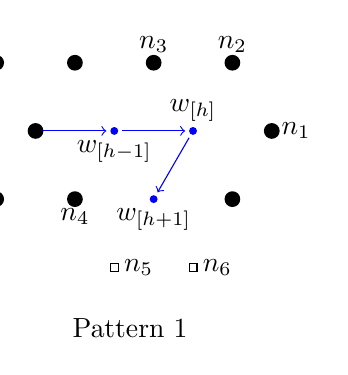
\begin{tikzpicture}

          \fill[transform canvas={shift=(0:0)}](0,0) circle [radius=0.1];
          
          \foreach \theta in {60,-60,120,-120,180}{
            \fill[transform canvas={shift=(\theta:1)}](0,0) circle [radius=0.1];
          }

          \fill[blue](0:1) circle [radius=0.05];
          \draw[->, blue] (0:0.1)--(0:0.9);

          \node[below] at (-60:1) {$n_4$};

          \begin{scope}[shift=(0:2)]
            \fill[blue](0,0) circle [radius=0.05];

            
            \foreach \theta in {120,60,-60,0}{
             \fill[transform canvas={shift=(\theta:1)}](0,0) circle [radius=0.1];
            }

            \draw[->, blue] (180:0.9)--(180:0.1);
            \draw[->, blue] (-120:0.1)--(-120:0.9);

            \node[below] at (180:1) {$w_{[h-1]}$};
            \node[above] at (0:0) {$w_{[h]}$};
            \node[below] at (-120:1) {$w_{[h+1]}$};

            \node[above] at (120:1) {$n_3$};
            \node[above] at (60:1) {$n_2$};
            \node[right] at (0:1) {$n_1$};

            \begin{scope}[shift=(-120:1)]
              \fill[blue](0,0) circle [radius=0.05];
              \foreach \theta in {-120,-60}{
                \draw[transform canvas={shift=(\theta:1)}](-0.05,-0.05) rectangle (0.05,0.05);
              }

              \node[right] at (-120:1) {$n_5$};
              \node[right] at (-60:1) {$n_6$};
            \end{scope}
            
          \end{scope}

          \node at (1.2,-2.5) {Pattern 1};
        \end{tikzpicture}
      \end{minipage}

      \begin{minipage}{0.48\hsize}
      \centering
        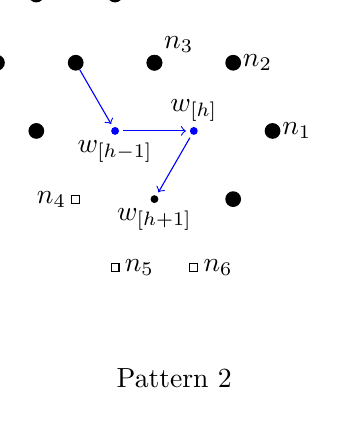
\begin{tikzpicture}

          \fill(0,0) circle [radius=0.1];
          
          \foreach \theta in {60,0,120,-120,180}{
            \fill[transform canvas={shift=(\theta:1)}](0,0) circle [radius=0.1];
          }

          \draw[->, blue] (-60:0.1)--(-60:0.9);


          \begin{scope}[shift=(-60:1),shift=(0:1)]
            \fill[blue](0,0) circle [radius=0.05];
            \fill[blue](180:1) circle [radius=0.05];

            
            \foreach \theta in {120,60,0,-60}{
              \fill[transform canvas={shift=(\theta:1)}](0,0) circle [radius=0.1];
            }

            \draw[->, blue] (180:0.9)--(180:0.1);
            \draw[->, blue] (-120:0.1)--(-120:0.9);

            \node[below] at (180:1) {$w_{[h-1]}$};
            \node[above] at (0:0) {$w_{[h]}$};
            \node[below] at (-120:1) {$w_{[h+1]}$};

            \node[above right] at (120:1) {$n_3$};
            \node[right] at (60:1) {$n_2$};
            \node[right] at (0:1) {$n_1$};

            \begin{scope}[shift=(-120:1)]
              \fill(0,0) circle [radius=0.05];
              \foreach \theta in {180,-120,-60}{
                \draw[transform canvas={shift=(\theta:1)}](-0.05,-0.05) rectangle (0.05,0.05);
              }

              \node[left] at (180:1) {$n_4$};
              \node[right] at (-120:1) {$n_5$};
              \node[right] at (-60:1) {$n_6$};
            \end{scope}
            
          \end{scope}

          \node at (1.25,-4) {Pattern 2};
        \end{tikzpicture}
      \end{minipage}

      
      
    \end{tabular}
    \caption{Case of $S[h-1..h+1] = tbt$}
    \label{TTT_tunnelC_enter_usingTunnel}
\end{figure}



%\end{proof}



%%%%%%%%%%%%%%%%%%%%%%%%%%%%%%%%%%%%%%%%%%%%%%%%%%%%
%%
%%%%
%%%%%%
%%%%%%%%
%%%%%%%%%%%%%%%%%%%%%%%%%%%%%%%%%%%%%%%%%%%%%%%%%%%%

\proof{Proof of Tunnel Troll Theorem}
%Each bead in the transcript is bound either inside a tunnel or outside. If a bead is stabilized inside a tunnel, 
%then it has at most one free neighbor, and hence its successor it to be stabilized there.
%Moreover, if a bead is stabilized outside a tunnel, then its position is either an entrance of a tunnel or not.
%
%Tunnel sections have three possible shapes up to symmetry : straight($S$), obtuse($O$) and acute($A$) turn (Fig. \ref{fig:TTT_tunnel}), and we will consider each of those. 


%\begin{lemma}
%\label{TTT_neighbor_lemma}
%For unary transcripts at $\delta = 1$, if a bead has no free hand, then at least $\alpha + 2$ of its neighbors have to be occpied.
%\end{lemma}

Let us first consider cases of $\delta \geq 3, \alpha = 1$. 
See Fig.~\ref{TTT_tunnel_exit}. Consider the stabilization of $w[i]$. 
This bead $w[i]$, once stabilized, shares two neighbors with its predecessor $w[i-1]$, which are denoted by $n_3, n_4$. 
Both of them have been already occupied because $S[i] = t$. 

Since $S[i+1] \neq \blacksquare$, at least one of the other three neighbors, denoted by $n_0, n_1, n_2$, must be free. 
Assume that in the neighborhood of $w[i]$, there are two beads with one free neighbor even after $w[i]$ is stabilized. 
Before the stabilization of $w[i]$, such a bead had two free neighbors, and hence, is provided with at least one free bond. 
Thus, $w[i]$ is to be bonded to these two beads, and it decreases the binding capability by at least 1. 
It now suffices to check that this assumption holds no matter how $n_0, n_1, n_2$ are occupied as long as at least one of them is left free. 

Next, we consider the case of $\delta = 2, \alpha = 1$. We assume there are an indices $i$ ,$j$ such that $S[i+1..j+1] = bt^{(j-i-1)}b$ and $S[i+2] \in \{ t_s, t_o \} $.
Then, all $S[i+1..j]$ do not contain $t_o$; otherwise $S[i+1..j]$ contain $\blacksquare$.
Therefore according to Lemma~\ref{TTT_entrance_Tab}, $\#bc(C_{i-1}) > \#bc(C_{i})$ and moreover that, according to Lemma~\ref{TTT_exit}, $\#bc(C_{i}) \geq \#bc(C_{j})$.


On the other hand, we assume there are an indices $i$ ,$j$ such that $S[i+1..j+1] = bt^{(j-i-1)}b$ and $S[i+2] = t_a$.


Let us consider that $w[i]$ supplies two bonds (that is, $S[i] = t$).
If $S[i] \in \{ t_s, t_o \}$, $\#bc(C_{i-2}) \geq \#bc(C_{i})$ because of Lemma~\ref{TTT_exit}.
Therefore, 

if $S[k..l] = bt^{l-k}b$, then $\#bc(C_{k-1}) \geq \#bc(C_{l})$ because of Lemma~\ref{TTT_exit}. Therefore, if there are indices $i$ and $j$ such that $S[i..j+1] = bbt^{(j-i-1)}b$ or $S[i..j+1] = bt^mbt^nb \quad (m + n = j-i-1)$, then $\#bc(C_{i-1}) > \#bc(C_{j})$.

\qed






%%%%%%%%%%%%%%%%%%%%%%%%%%%%%%%%%%%%%%%%%%%%%%%%%%%%%%%%%
%/////////////////////////////////////////////////
%%%%%%%%%%%%%%%%%%%%%%%%%%%%%%%%%%%%%%%%%%%%%%%%%%%%%%%%%


\subsection{On structures provided by a unary and $\delta = 1$ oritatami system}

\begin{figure}[tb]
 \centering
    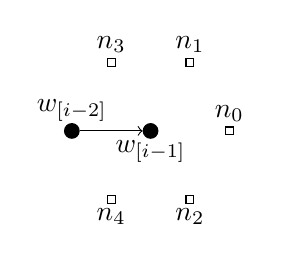
\begin{tikzpicture}
	\fill[shift=(180:1)] (0,0) circle [radius=0.1];
      \fill[shift=(180:0)] (0,0) circle [radius=0.1];
      
      \draw[->] (180:0.9) -- (180:0.1);

	\node[above] at (180:1) {$w_{[i-2]}$};
	\node[below] at (180:0) {$w_{[i-1]}$};
	\node[above] at (0:1) {$n_0$};

	\foreach \theta in {0,60,-60,120,-120}{
   	   \draw [shift=(\theta:1)] (-0.05,-0.05) rectangle (0.05,0.05);
  	}
 	\node[above] at (60:1) {$n_1$};
	\node[below] at (-60:1) {$n_2$};
	\node[above] at (120:1) {$n_3$};
	\node[below] at (-120:1) {$n_4$};
    \end{tikzpicture}
    \caption{$\alpha = 4$: when $w[i]$ is stabilized}
    \label{TTT_a4_lemma_fig}
\end{figure}

%\begin{lemma}
%\label{TTT_a4_2b_lemma}
%Let $\Xi$ be a deterministic unary oritatami system of $\delta = 1, \alpha = 4$.
%When a bead is stabilized by bond, it forms at least two bonds.
%\end{lemma}
%
%\begin{proof}%[proof of lemma]
%Suppose $w[i]$ were stabilized by only one bond. See Fig.~\ref{TTT_a4_lemma_fig}. If $n_3$ is free, $w[i-2]$ still has some bonds because of arity $\alpha = 4$. Thus, $n_4$ must be occupied; otherwise, $w[i]$ would be stabilized nondeterministically at $n_3$ and $n_4$. Moreover, also $n_2$ has to be occupied for deterministic and also $n_0, n_1$. $n_1$ has some hands because $n_3$ is free. Therefore, $w[i]$ is stabilized at $n_3$ and it has to use at least two hands. It contradict assumption.
%\end{proof}



\begin{figure}[tb]
 \centering
    \begin{tikzpicture}

	\fill (0,0) circle [radius=0.1];
        \fill[blue] (60:1) circle [radius=0.05];
        \fill (0:1) circle [radius=0.1];
      
      \draw[dashed] (180:2) -- (0:2);
      \draw[dashed, shift=(60:1)] (180:2.5) -- (0:1.5);
      \draw[->, blue] (60:0.1) -- (60:0.9);

	\node[above] at (180:1) {$p_1$};
	\node[left] at (-120:1) {$p_2$};
	\node[left] at (-60:1) {$p_3$};
	\node[left, shift=(-120:1)] at (-60:1) {$p_3$};

	\draw (180:1) circle [radius=0.05];
	\draw (-120:1) circle [radius=0.05];
	\draw (-60:1) circle [radius=0.05];
	\draw[shift=(-120:1)] (-60:1) circle [radius=0.05];

	\node at (0:2.5) {$n$};
	\node[shift=(60:1)] at (0:2) {$n+1$};
    \end{tikzpicture}
    \caption{the first bead out of $\hexagon_{w[-n+1]}^n$}
    \label{TTT_a4_first}
\end{figure}

\begin{theorem}[$\delta = 1, \alpha = 4$]
Let $\Xi$ be a deterministic unary oritatami system of $\delta = 1, \alpha = 4$. It can yield only finite conformation of length is $3n^2  + 3n + 1$.
\end{theorem}

\begin{proof}
Consider the moment when a bead $b$ is stabilized outside $\hexagon_O^n$ for the first time. 
See Fig.~\ref{TTT_a4_first}
There is only one bead available to stabilize $b$ there, which is $b_1$. 
In order for $b$ to avoid nondeterminism, hence, none of the beads around should not attract $b$. 

The point $p_1$ must be empty because a bead there would have at least two free neighbors and hence is provided with a free hand. 
If there is a bead at $p_2$, $n$ must be at least 2 so that the bead is not singular. 
Since $p_1$ is empty, this bead has at least one free hand, a contradiction. 
Thus, $p_2$ must be also empty. 
In the same way, we can easily show that the point $p_3$ must not be occupied by a non-singular bead. 
Suppose $p_3 = O$. 
The point $p_4$ must not be empty; otherwise the singular bead, at $O$, would have a free hand. 
However, then a bead at $p_4$ would be provided with a free hand, a contradiction. 
\qed
\end{proof}





%\begin{lemma}
%\label{TTT_a3_2b_lemma}
%Let $\Xi$ be a deterministic unary oritatami system of $\delta = 1, \alpha = 3$. 
%If $S[i] = t$ or $t^\times$ and $S[i+1] \neq \blacksquare$, then the bead $w[i]$ consumes also at least one bond. 
%% Let $p$ be a point whose neighbors is occupied at least two point. If $w[i]$ is not stabilized and $w[i-1]$ includes neighbors of $p$, then $w[i]$ is stabilized at $p$ with at least one bond, $w[i]$ is stabilized at another point of $p$ otherwise with at least two bond except any neighbors of $p$ is occupied.
%\end{lemma}
%
%\begin{proof}%[proof of lemma]
%Both $n_3$ and $n_4$ are occupied because $S[i] = t$ or $t^\times$.
%Suppose $w[i]$ were stabilized without any bond.
%Then, all neighbors of $n_3$ must be occupied as long as the bead at $n_3$ is not singular; otherwise, a bead at $n_3$ would be capable of forming a bond with $w[i]$.
%That is, $n_1$ is occupied.
%We can continue this argument in clockwise manner to fill the neighbors of $w[i]$ until a singular bead is encountered, if any.
%If needed, the same argument is applied starting from $n_4$ in counter-clockwise manner.
%Thus, all neighbors of $w[i]$ must be occupied but then $S[i+1] = \blacksquare$, contradiction. \qed
%\end{proof}


\begin{figure} [tb]
  \begin{center}
  \begin{tabular}{c c c}
 \begin{minipage}{0.3\hsize}
 \centering
    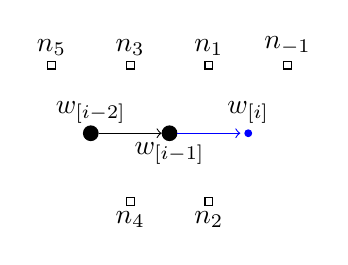
\begin{tikzpicture}
      
      \fill[shift=(180:1)] (0,0) circle [radius=0.1];
      \fill[shift=(180:0)] (0,0) circle [radius=0.1];
      
      \fill[blue](0:1) circle [radius=0.05];
      
      \draw[->] (180:0.9) -- (180:0.1);
      \draw[->, blue] (0:0.1) -- (0:0.9);

	\node[above] at (180:1) {$w_{[i-2]}$};
	\node[below] at (180:0) {$w_{[i-1]}$};
	\node[above] at (0:1) {$w_{[i]}$};

	\foreach \theta in {60,-60,120,-120}{
   	   \draw [shift=(\theta:1)] (-0.05,-0.05) rectangle (0.05,0.05);
  	}
	 \draw [shift=(60:1)] (0.95,-0.05) rectangle (1.05,0.05);
	  \draw [shift=(180:1),shift=(120:1)] (-0.05,-0.05) rectangle (0.05,0.05);
 	\node[above] at (60:1) {$n_1$};
	\node[below] at (-60:1) {$n_2$};
	\node[above] at (120:1) {$n_3$};
	\node[below] at (-120:1) {$n_4$};
	\node[above, shift=(0:1)] at (60:1) {$n_{-1}$};
	\node[above, shift=(180:1)] at (120:1) {$n_5$};
    \end{tikzpicture}
    \end{minipage}
    
    \begin{minipage}{0.3\hsize}
    \centering
     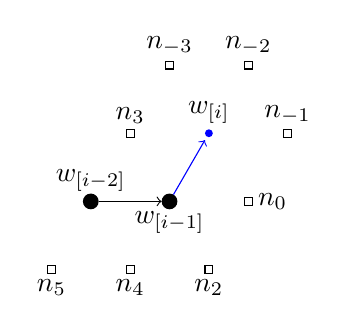
\begin{tikzpicture}
      
      \fill[shift=(180:1)] (0,0) circle [radius=0.1];
      \fill[shift=(180:0)] (0,0) circle [radius=0.1];
      
      \fill[blue](60:1) circle [radius=0.05];
      
      \draw[->] (180:0.9) -- (180:0.1);
      \draw[->, blue] (60:0.1) -- (60:0.9);

	\node[above] at (180:1) {$w_{[i-2]}$};
	\node[below] at (180:0) {$w_{[i-1]}$};
	\node[above] at (60:1) {$w_{[i]}$};


	\foreach \theta in {0,-60,120,-120}{
   	   \draw [shift=(\theta:1)] (-0.05,-0.05) rectangle (0.05,0.05);
  	}
	\draw [shift=(60:1)] (0.95,-0.05) rectangle (1.05,0.05);
	\draw [shift=(60:1), shift=(60:1)] (-0.05,-0.05) rectangle (0.05,0.05);
	\draw [shift=(60:1), shift=(120:1)] (-0.05,-0.05) rectangle (0.05,0.05);
	  \draw [shift=(180:1),shift=(-120:1)] (-0.05,-0.05) rectangle (0.05,0.05);
	
 	\node[right] at (0:1) {$n_0$};
	\node[below] at (-60:1) {$n_2$};
	\node[above] at (120:1) {$n_3$};
	\node[below] at (-120:1) {$n_4$};
	\node[above, shift=(60:1)] at (0:1) {$n_{-1}$};
	\node[above, shift=(60:1)] at (60:1) {$n_{-2}$};
	\node[above, shift=(60:1)] at (120:1) {$n_{-3}$};
	\node[below, shift=(180:1)] at (-120:1) {$n_5$};
    \end{tikzpicture}
    \end{minipage}
    
    \begin{minipage}{0.3\hsize}
        \centering
     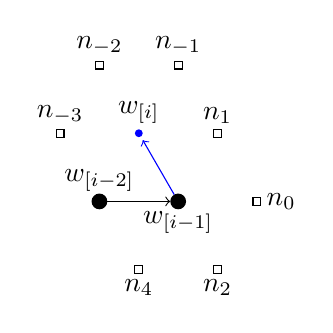
\begin{tikzpicture}
      
      \fill[shift=(180:1)] (0,0) circle [radius=0.1];
      \fill[shift=(180:0)] (0,0) circle [radius=0.1];
      
      \fill[blue](120:1) circle [radius=0.05];
      
      \draw[->] (180:0.9) -- (180:0.1);
      \draw[->, blue] (120:0.1) -- (120:0.9);

	\node[above] at (180:1) {$w_{[i-2]}$};
	\node[below] at (180:0) {$w_{[i-1]}$};
	\node[above] at (120:1) {$w_{[i]}$};


	\foreach \theta in {0,60,-60,-120}{
   	   \draw [shift=(\theta:1)] (-0.05,-0.05) rectangle (0.05,0.05);
  	}
	\draw [shift=(120:1), shift=(60:1)] (-0.05,-0.05) rectangle (0.05,0.05);
	\draw [shift=(120:1), shift=(120:1)] (-0.05,-0.05) rectangle (0.05,0.05);
	\draw [shift=(120:1), shift=(180:1)] (-0.05,-0.05) rectangle (0.05,0.05);
	
 	\node[right] at (0:1) {$n_0$};
	\node[above] at (60:1) {$n_1$};
	\node[below] at (-60:1) {$n_2$};
	\node[below] at (-120:1) {$n_4$};
	\node[above, shift=(120:1)] at (60:1) {$n_{-1}$};
	\node[above, shift=(120:1)] at (120:1) {$n_{-2}$};
	\node[above, shift=(120:1)] at (180:1) {$n_{-3}$};
    \end{tikzpicture}
    \end{minipage}
    \end{tabular}
    \caption{All possible directions of $w[i]$: straight, obtuse, acute.}
    \label{TTT_a3_w}
  \end{center}
\end{figure}

\begin{theorem}[$\delta = 1, \alpha = 3$]
Let $\Xi$ be a deterministic unary oritatami system of $\delta = 1, \alpha = 3$. It can yield only finite conformations of length is $O(n)$.
\end{theorem}

%Both $n_3$ and $n_4$ are occupied because $S[i] = t$ or $t^\times$.
%Suppose $w[i]$ were stabilized without any bond.
%Then, all neighbors of $n_3$ must be occupied as long as the bead at $n_3$ is not singular; otherwise, a bead at $n_3$ would be capable of forming a bond with $w[i]$.
%That is, $n_1$ is occupied.
%We can continue this argument in clockwise manner to fill the neighbors of $w[i]$ until a singular bead is encountered, if any.
%If needed, the same argument is applied starting from $n_4$ in counter-clockwise manner.
%Thus, all neighbors of $w[i]$ must be occupied but then $S[i+1] = \blacksquare$, contradiction. \qed


\begin{proof}
We consider cases which $w[i-1]$ is two distances away from the singular point.
Let us show that $\#bc(C_{i-1}) > \#bc(C_i)$, that is, when $w[i]$ is stabilized, $w[i]$ uses at least two hands.
Fig.\ref{TTT_a3_w} exhibits all the three kinds of possibility of stabilized $w[i]$.
Suppose $w[i]$ were able to be stabilized with using one hand in each cases.

% Then, $w[i]$ can be also stabilized at $n_3$. 

\begin{paragraph}{Case of straight}
\begin{itemize}
\item[-] Case of $n_3$ is free\\
The bead $w[i-2]$ must not have bonds because $w[i]$ is stabilized deterministically so that five neighbors of $w[i-2]$ must be occupied.
Therefore $n_5$ must be occupied.
We can continue this argument in clockwise manner to fill the neighbors of $n_3$ until $n_1$.
However, two neighbors of $n_1$ must be free because they are $n_3$ and the point of $w[i]$, contradict.

\item[-] Otherwise\\
Both $n_3$ and $n_4$ are occupied.
One of $n_1$ and $n_2$ must be free because $S[i] = b$.
We assume $n_1$ is free, then all neighbors of $n_1$ must be occupied because $n_3$ is occupied.
However, one of neighbors $n_1$ is a point which $w[i]$ is stabilized, contradict.
\end{itemize}

Therefore, this case contradict assumption.
\end{paragraph}

\begin{paragraph}{Case of obtuse}
\begin{itemize}
\item[-] Case of $n_3$ is free\\
Any neighbors of $n_3$ have to be occupied but the point which $w[i]$ is stabilized is free. Thus $n_3$ has to be occupied.
\item[-] Case of $n_4$ is free\\
The point $n_2$ must be occupied because $n_4$ is free and $n_5$ must be occupied.
Therefore $n_0$ is occupied.
The bead $w[i]$ forms just one bond so that one of $n_0, n_3$ leave some hands or both of them do not leave any bonds.\\
If $n_0$ has some hands, then $n_3$ does not have any hands so that $n_{-3}$ is occupied. 
We can continue this argument in clockwise manner to fill the neighbors of $w[i]$.
That is, $S[i] = \blacksquare$, contradict.

If $n_3$ has some hands, then $n_0$ does not have any hands so that neighbors of $w[i]$ are occupied. In the same previous way, contradict.\\
If both of $n_0, n_3$ do not have any hands, then both of $n_{-1}, n_{-3}$ are occupied. If one of $n_{-1}, n_{-3}$ has some hands, the other does not have any hands so that $n_{-2}$ is occupied. If both of $n_{-1}, n_{-3}$ do not have any hands, $n_{-2}$ has to be occupied and $n_{-2}$ has some hands, contradict.
\item[-] Case of $n_2$ is free\\
Any neighbors of $n_2$ have to be occupied so that $n_0$ is occupied. Any neighbors of $n_0$ except $n_2$ have to be also occupied but the point which is stabilized $w[i]$ is free. Thus $n_2$ has to be occupied.
\item[-] Case of $n_0$ is free\\
Any neighbors of $n_0$ have to be occupied so that $n_{-1}$ is occupied. Any neighbors of $n_{-1}$ except $n_0$ have to be also occupied but the point which is stabilized $w[i]$ is free. Thus $n_0$ has to be occupied. 
\end{itemize}
\end{paragraph}



\begin{paragraph}{Case of acute}
\begin{itemize}
\item[-] Case of $n_4$ is free\\
The point $n_4$ and a point which is stabilized $w[i]$ are free so that  $w[i-2]$ has some bonds.
However, $w[i]$ can be also stabilized $n_4$ in this case. Thus, $n_4$ has to be occupied.
\item[-] Case of $n_2$ is free\\
The point $n_0$ has to be occupied. The point $n_1$ has to be also occupied because five neighbors of $n_0$ must be occupied.
We consider this case just like case of obtuse and that $n_4$ is free. Then if $w[i-2]$ binds $w[i]$, any $n_{-1}, n_{-2}, n_{-3}$ are occupied. If $n_1$ binds $w[i]$, this case is same. Also if $n_1$ and $w[i-2]$ do not have any hand, any $n_{-1}, n_{-2}, n_{-3}$ are occupied. Therefore, $w[i+1]$ cannot be provided.
\item[-] Case of $n_0$ is free\\
Any neighbors of $n_0$ have to be occupied so that $n_{1}$ is occupied. Any neighbors of $n_{1}$ except $n_0$ have to be also occupied but the point which is stabilized $w[i]$ is free. Thus $n_0$ has to be occupied. 
\item[-] Case of $n_1$ is free\\
Any neighbors of $n_1$ have to be occupied so that $n_{-1}$ is occupied. Any neighbors of $n_{-1}$ except $n_1$ have to be also occupied but the point which is stabilized $w[i]$ is free. Thus $n_1$ has to be occupied. 
\end{itemize}

Therefore, any situations contradict $S[i] = b$.
\end{paragraph}\\


Hence, $w[i]$ uses at least two bonds if $w[i-1]$ is at least two distances away the singular point.
The size of $ \hexagon^2_0 = 19$ and this number contain the singular point, its successor and its three neighbors which is it binds to. Therefore 14 times  $w[i]$ can be stabilized by forming one bond.
Therefore, a deterministic unary oritatami system at $\delta = 1$ and $\alpha = 3$ can yield only finite conformation of length is $2n + 14$.
\end{proof}




\begin{theorem}[$\delta= 1, \alpha=2$]
Let $\Xi$ be a unary oritatami system of $\delta = 1, \alpha = 2$. It can yield infinite structures but they are only zig-zag conformation.
\end{theorem}

\begin{proof}
By Tunnel Troll Theorem, any tunnel sections which represented in $bbt^+$ or $bt^+bt^+$ consume binding capabilities. If the sequence $S$ is free from any subsequence of the form $bt^+bt^+$, then it can factorize as $S = u_1 u_2 u_3 \cdots$ for some $u_1 , u_2 , u_3 , \cdots \in \{b\} \cup bbt^+$. Assume the length of $\sigma$ is $n$, seed supplies at most $2n$ binding capabilities. Therefore formula \ref{TTT_only_bond} hold.

\begin{eqnarray}
  \exists i \in \mathbb{N} \quad s.t. \quad u_{i-1} , u_i , u_{i+1} , u_{i+2} , \cdots \in \{ b \}
  \label{TTT_only_bond}
\end{eqnarray}


Let us represent $S$ as $S[i.i+1...] = v_i v_{i+1} v_{i+2} \cdots$ for some $v_i, v_{i+1}, v_{i+2}, \cdots \in \{ a, o\}$ where if $v_k$ is $a$, then $v_{k+1}$ is bound to $v_{k-1}$, if $v_k$ is $o$, then $v_{k+1}$ is NOT bound to $v_{k-1}$.


Let us consider the case of $v_k$ is $o$. See Fig.\ref{TTT_case_of_o}. $w[i-1]$ consumes some binding capabilities because $v_{i-1}$ is $b$. If the number of $w[i-1]$'s bindings is one binding, then $w[i+1]$ has to be bound except $n_1$ or $n_2$ so that $w[i+1]$ must consumes two bindings except the case of $n_1$ and $n_2$ are occupied and $w[i]$ consumes at least one binding. If $n_1$ and $n_2$ are occupied, then $w[i-1]$'s bindings are inactive, that is, $w[i-1]$ consumes two binding capabilities. Therefore, this case consumes binding capabilities. If $w[i-1]$ dose Not have any bindings, then $w[i-1]$ already consumes two bindings. In addition, $w[i]$ and $w[i+1]$ consume at least one binding. Therefore this case consumes binding capabilities. Thus, the formula \ref{TTT_only_a} hold and according to the formula \ref{TTT_only_bond} and the formula \ref{TTT_only_a}, the formula \ref{TTT_structure} is hold. Thus, in this case, oritatami system can yield infinite structures but they are only zig-zag conformation.

\end{proof}

\begin{eqnarray}
  \exists j \in \mathbb{N} \quad s.t. \quad u_j , u_{j+1} , u_{j+2} , \cdots \in \{ a \}
  \label{TTT_only_a}
\end{eqnarray}

\begin{eqnarray}
  | S | > \forall m \in \mathbb{N} \quad \to \quad \exists n \in \mathbb{N} \quad s.t. \quad S[n], S[n+1], \cdots \in \{ a \}
  \label{TTT_structure}
\end{eqnarray}

\begin{figure}
  \begin{center}
    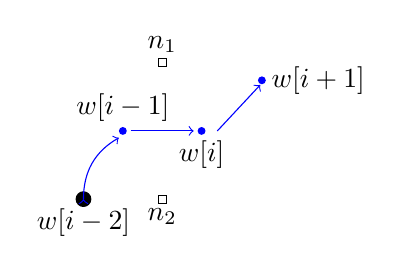
\begin{tikzpicture}
      
      \fill[transform canvas={shift=(-120:1)}](0,0) circle [radius=0.1];
      
      \fill[blue](0:0) circle [radius=0.05];
      \fill[blue](0:1) circle [radius=0.05];
      \fill[shift=(0:1), blue](40:1) circle [radius=0.05];

      \draw[->, blue] (-120:1) edge[bend left] (-120:0.1);
      \draw[->, blue] (0:0.1) -- (0:0.9);
      \draw[->,transform canvas={shift=(0:1.2)}, blue] (50:0) -- (47:0.8);
      
      \draw[shift=(60:1)](-0.05,-0.05) rectangle (0.05,0.05);
      \draw[shift=(-60:1)](-0.05,-0.05) rectangle (0.05,0.05);
      
      \node[below] at (-120:1) {$w[i-2]$};
      \node[above] at (0:0) {$w[i-1]$};
      \node[below] at (0:1) {$w[i]$};
      \node[right, shift=(0:1)] at (40:1) {$w[i+1]$};

      \node[above] at (60:1) {$n_1$};
      \node[below] at (-60:1) {$n_2$};
        
    \end{tikzpicture}
    \caption{Case of $S[i]$}
    \label{TTT_case_of_o}
  \end{center}
\end{figure}




